\subsection{La boucle \texttt{while}}

La boucle \texttt{while} est un outil très puissant en programmation. En français, cela correspond à dire \textit{tant que cette condition est vraie, j'exécute le code suivant}. En informatique, cela s'écrit avec le mot \texttt{while} suivi d'une expression booléenne et de \texttt{:}.
\subsubsection{Fonctionnement}
\begin{enumerate}
\item On évalue l'expression booléenne
\item Si l'expression est \textbf{False} : on ignore le code indenté qui suit le \textbf{while}.
\item Si l'expression est \textbf{True} : on exécute le code indenté qui suit \textbf{while} et retour à l'étape 1.
\end{enumerate} 
\begin{python}[caption = Exemple de boucle while]
"""Affiche tous les nombres de la table de 9 plus petits que 100"""
i = 0
while i <= 100:
	print("i vaut " + str(i))
	i = i+9	# Mise a jour de i
print("Fini")
\end{python}

\subsubsection{Attention à la boucle infinie!}

Comme vous avez pu le voir, la (ou les) variable de l'expression booléenne est mise à jour dans la boucle \texttt{while}. Dans le cas contraire, on ne sortira jamais de la boucle puisque la valeur de la condition de celle-ci ne sera jamais changée. Cet oubli de mise à jour crée ce qu'on appelle des boucles infinies et sont une erreur très courante. Ces dernières, en fonction de l'endroit où elle surgissent, peuvent faire planter votre programme.

\begin{python}[caption = Exemple de boucle infinie]
i = 0
while i < 10:
	print "Je suis dans la boucle"
print "Ce message ne s'affichera jamais"
\end{python}

\begin{figure}[!h]
    \centering
    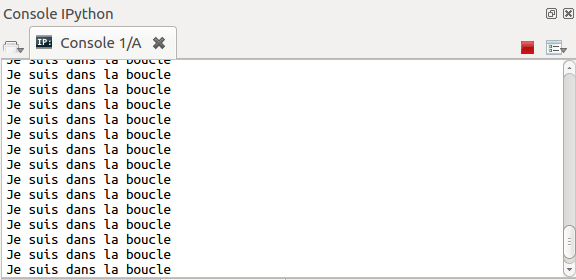
\includegraphics[width=7cm]{boucle_inf.png}
    \caption{Le programme ne s'arrête jamais}
    \label{arbre}
\end{figure}

\subsection{La boucle \texttt{for}}

La boucle \texttt{for} est, elle aussi, un réel passe-partout\footnote{Attention pas le même que celui de Fort-Boyard !} du programmeur. En \textsc{Python}, elle permet d'appliquer un code (\textit{indenté}) à chaque élément d'une structure de données\footnote{Par exemple un String ou une liste}. Elle commence toujours par le premier élément de la structure et finit par le dernier.

Pour ce faire, on écrit : \lstinline{for i in ma_structure}. Ici \texttt{i} (notez qu'on pourrait très bien choisir un autre nom de variable) est appelé \textit{itérateur}, c'est-à-dire que c'est lui qui prendra successivement la première valeur de la structure de données, puis la seconde, et ainsi de suite.

\begin{python}[caption = la boucle for]
"""Utilise une boucle for pour imprimer un string"""
s = "Hello World"
for i in s:
	print i
print "done" 
\end{python}

\subsection{Le \texttt{break}}
On peut, si on le désire, sortir à tout moment d'une boucle. Pour ce faire, on utilise le mot clé \textbf{break} à l'endroit où l'ont veut sortir. 

\begin{python}
i = 0
while(i<100):
	if i != 50:
		print i
		i = i+1
	else:
		break
\end{python}

\textbf{Attention : } un \texttt{break} est considéré comme une sortie "sale" d'une boucle. On ne l'utilise donc que lorsque cela est absolument nécessaire !

\subsection{Exercices : }
\begin{enumerate}
\item \textbf{Exercice 1 : } Améliorez votre convertisseur de l'exercice \ref{convertisseur} pour qu'il convertisse les unités de l'utilisateur jusqu'à ce que celui entre le mot "stop".  

\item \textbf{Exercice 2 : } Implémentez un programme qui prend un texte en entrée (fourni par l'utilisateur) et imprime chaque voyelle du texte. (Essayez avec un texte très long trouvé sur Internet...)

\item \textbf{Exercice 3 : } Implémentez un programme qui prend un texte en entrée (fourni par l'utilisateur) et qui imprime \textbf{True} si le texte contient un palindrome et \textbf{False} sinon. (\textbf{Aide :} un palindrome est un mot qui peut se lire dans les 2 sens. \textit{Exemple} : kayak, abcba, ...)
\end{enumerate}